\documentclass[conference]{IEEEtran}
\PassOptionsToPackage{dvipsnames}{xcolor}
\usepackage[utf8]{inputenc} % To use Unicode (e.g. Turkish) characters
\usepackage[T1]{fontenc}
\renewcommand{\labelenumi}{(\roman{enumi})}
\usepackage{amsmath, amsthm, amssymb}
 % Some extra symbols
\usepackage[bottom]{footmisc}
\usepackage{cite}
\usepackage{graphicx}
\usepackage{algorithm,algorithmicx,algpseudocode}
\usepackage{dcolumn}
\usepackage{listings}

\usepackage{url}
\usepackage{multicol}
\usepackage{longtable}
\usepackage{xargs}
\usepackage{booktabs}
%
\usepackage[colorinlistoftodos,prependcaption,textsize=tiny]{todonotes}
\graphicspath{{figs/}} % Graphics will be here

\usepackage{multirow}
\usepackage{subcaption}
\usepackage{float}
%\usepackage[linesnumbered,ruled,vlined]{algorithm2e}

\usepackage{soul}
\usepackage{adjustbox}
\usepackage{svg}

\DeclareRobustCommand{\fba}[1]{ {\begingroup\sethlcolor{BurntOrange}\hl{(fba:) #1}\endgroup} }

\usepackage[super]{nth}
\usepackage[framemethod=tikz]{mdframed}

\newmdenv[bottomline=false, linecolor=black!60!black, innertopmargin=0.1cm,innerleftmargin=0.1cm,innerbottommargin=0.1cm]{bottomless}
\newfloat{lstfloat}{htbp}{lst}
\floatname{lstfloat}{Listing}

\newenvironment{breakablealgorithm}
  {% \begin{breakablealgorithm}
   \begin{center}
     \refstepcounter{algorithm}% New algorithm
     \hrule height.8pt depth0pt \kern2pt% \@fs@pre for \@fs@ruled
     \renewcommand{\caption}[2][\relax]{% Make a new \caption
       {\raggedright\textbf{\ALG@name~\thealgorithm} ##2\par}%
       \ifx\relax##1\relax % #1 is \relax
         \addcontentsline{loa}{algorithm}{\protect\numberline{\thealgorithm}##2}%
       \else % #1 is not \relax
         \addcontentsline{loa}{algorithm}{\protect\numberline{\thealgorithm}##1}%
       \fi
       \kern2pt\hrule\kern2pt
     }
  }{% \end{breakablealgorithm}
     \kern2pt\hrule\relax% \@fs@post for \@fs@ruled
   \end{center}
  }

\makeatletter
\newcounter{phase}[algorithm]
\newlength{\phaserulewidth}
\newcommand{\setphaserulewidth}{\setlength{\phaserulewidth}}
\newcommand{\phase}[1]{%
  \vspace{-1.25ex}
  % Top phase rule
  \Statex\leavevmode\llap{\rule{\dimexpr\labelwidth+\labelsep}{\phaserulewidth}}\rule{\linewidth}{\phaserulewidth}
  \Statex\strut\refstepcounter{phase}\textit{Phase~\thephase~--~#1}% Phase text
  % Bottom phase rule
  \vspace{-1.25ex}\Statex\leavevmode\llap{\rule{\dimexpr\labelwidth+\labelsep}{\phaserulewidth}}\rule{\linewidth}{\phaserulewidth}}
\makeatother


\algnewcommand{\LineComment}[1]{\State \(\#\) #1}



\begin{document}


\title{Visualizing Software Repositories through Rewuirements Trace Links}
% \author{
%  \IEEEauthorblockN{Kadir Ersoy, Ecenur Sezer, Suzan Üsküdarlı, Fatma Başak Aydemir}
% \IEEEauthorblockA{
% Boğaziçi University\\
% Istanbul, Türkiye \\
% \{kadir.ersoy, ecenur.sezer, suzan.uskudarli, basak.aydemir\}@boun.edu.tr}
% }

\author{
  \IEEEauthorblockN{Anonymous Authors}\\
\IEEEauthorblockA{Anonymous}}

%\date{May 2021}

\maketitle
\begin{abstract}
  % context
  Tracking the status of the requirements throughout the software development cycle is essential to the success of software development projects.
  % context
 %Requirements traceability refers to the capability of following the life of a requirement in both forwards and backward directions, and to the ability to link requirements to other software artifacts through particular relationships.
 % Motivation
  Requirements trace links relate requirements with other software development artifacts which indicates the progress on their related requirements. Manually identifying these trace links, and  understanding and aggregating them as an indicator of the requirement progress is a saunting task.
  %These traceability links enable stakeholders to monitor the development progress of requirements and assist system engineers in tracking the effort and workload associated with fulfilling those requirements.
  % Approach
  % Traditional methods to recover traceability links necessitate significant human effort, making them unsuitable and inefficient, particularly as the project scale grows.
  % Approach
  This paper implements and evaluates trace links from requirements to issues, pull requests, and commits using keyword matching, TF-IDF vectors and word vectors. Extracted links are used to create interactive visualization of the repository in a dashboard for retrospective and real-time analysis.
  % Results
  Our preliminary evaluation suggests that word vector method outperforms the other methods.
  % Contribution
  Our main contribution is the interactive dashboard that utilizes trace links to visualize a software repository to support project management and analysis. We also lay out details for our future evaluation plan. Our replication package contains the code and the evaluation data.
%In this work, we present a tool that establishes automated requirement traceability links between requirements written in natural language and software artifacts acquired from GitHub repositories. The tool implements three optional methods to trace the artifacts to the requirements, namely a keyword extraction pipeline, TF-IDF vector and word-vector. The captured traces are stored in a graph database and visualized. Additionally, an interactive dashboard featuring statistical data about the artifacts and their traces is implemented. By offering automated traceability and comprehensive visualization, this tool aims to enhance the management of requirements and to understand their quality in software development projects.
  %Contribution

\end{abstract}
\begin{IEEEkeywords}
  software management, repository visualization, requirements traceability, trace graph
\end{IEEEkeywords}


\section{Introduction}
\label{sec:intro}

% \begin{itemize}
%     \item Requirements traceability definition
%     \item Why do we do it, examples
%     \begin{itemize}
%         \item It is too hard to do it manually
%         \begin{itemize}
%             \item Cost of integration: Need trace link recovery,
%             \item Human effort: Do not force extra measures for traceability
%         \end{itemize}
%         \item Its role in project management
%         \begin{itemize}
%             \item Monitoring the progress: Status of the project
%             \item Effort assessment: How much effort went to which features
%             \item Detecting problems for specific features
%         \end{itemize}
%     \end{itemize}
%     \item showcasing trace data and other stats to user in a self-evident manner
% \end{itemize}

Requirements traceability refers to the capability of following the life of a requirement in both forwards and backward directions~\cite{gotel-1994}, and to the ability to link requirements to other software artifacts through particular relationships. Requirement traceability is crucial in software development projects since it shows the progress done in implementing the requirements and assists engineers in observing the effort and workload associated with them. All these aspects of requirement traceability help teams to ensure the fulfillment of specified requirements, by linking them to other software artifacts. Given that, it is a critical obstacle that traditional methods of recovering traceability links require significant time and human effort, making them unsuitable for the task as the project scale grows. Moreover, the quality of these methods is not consistent, since it highly depends on the understanding of the requirement traceability of the human analysts' performing them.
In this paper, we present a tool implemented to automate the process of identifying trace links. Our tool establishes links from requirements that are written in natural language to the software development artifacts, mainly Issues, PRs, and Commits, that are fetched from GitHub repositories. By automatizing this process, our tool aims to decrease the reliance on human effort and provides efficient requirement traceability management.

For identifying the trace links, three optional methods are implemented in our tool. These methods are keyword extraction, which performs keyword matching to software development artifacts, and TF-IDF Vector - Word Vector methods, which basically perform vector-based similarity. Each of these methods offers distinct advantages that are highly dependent on the context of the projects.
The software artifacts and the identified trace links are stored in a graph database and visualized in a graphical structure to enable efficient retrieval of traceability information. To improve the comprehension of the collected traceability data, our tool also features an interactive dashboard. This dashboard is equipped with valuable statistical insights about the lifetime of the project and the requirements. Along with the visualization of the traceability links and the offering of statistical data, we aim to improve the management of the requirements, ultimately leading to better-planned and programmed software projects.

The rest of the paper is structured as follows. Sec.~\ref{sec:relwork} presents the related work from the literature. Sec.~\ref{sec:approach} details our approach for identifying trace links. Our evaluation plan is described in Sec.~\ref{sec:eval}. Sec.~\ref{sec:discuss} discusses our findings. Finally, Sec.~\ref{sec:conc} concludes the paper and lays out the future work.

%\section{Problem and Motivation}
%\label{section:problem}

% Requirements traceability,
%     - definition,
% Why do we do it, examples
%     - It is too hard to do it manually
%     - Its role in project management,
%         - Monitoring the progress
%             - Status of the project
%             - What has been done
%         - Effort assessment
%             - How much effort went to which features
%         - Detecting problems for specific features
%             - In the case of a problem, look for it in a localized manner
%             - can be done since we know what has done for which context
%     - The use of requirements and req traceability is not common
%         - Cost of integration
%             - Need trace link recovery,
%         - Human effort
%             - Do not force extra measures for traceability
%     - To achieve wide-use of traceability
%         - user friendly,
%             - showcasing trace data and other stats to user in a self-evident manner
%         - minimal human effort,
%%% Local Variables:
%%% mode: latex
%%% TeX-master: "../main"
%%% End:
\section{Related Work}
\label{section:related_work}

There are several studies that focus on automating trace link recovery that implement various techniques. The common objective among the studies is to find relation between software artifacts, by performing diverse methods with various input and output types.

\subsection{Information Retrieval}

One of the popular approaches is to view trace link recovery as an information retrieval(IR) problem. Since the objective of IR, which is to find relevant documents in a document collection given a user query, is analogous to finding related software artifacts for a given requirement, it is very natural to approach the trace link recovery challenge as an information retrieval problem. More detailed information about IR can be found in\cite{IR}. Two of the widely adopted IR methods are vector-space model and probabilistic network model.

% \textbf{Vector-space model}

In vector-space model(VSM) method, each software artifact is represented by vectors. Thereby, the task of trace link recovery evolves into identifying vectors that are similar. Hayes et al.()\cite{hayes-2003} experimented with the vector-space model by examining three different version of it, a vanilla version, a version that incorporates technical terms and a version that uses a thesaurus for semantic association. They evaluated their methods on an open source NASA project, containing high level requirements with lower level requirement specifications. Provided in their evaluation, VSM almost always outperforms keyword-based methods and manual tracing in recall metric, but sometimes fails to do so in precision. They pointed out that even in the cases where VSM fails to outperform human analyst, it does perform faster. In a different study, Bonner et al. (2023)\cite{bonner-2023} have developed a tool that uses vector-space model to identify trace links between requirements and model-based designs. They have integrated their tool into the Siemens toolchain for Application Lifecycle Management(ALM).

% \textbf{Probabilistic-network model}

In probabilistic-network(PN) based model, a confidence score is calculated to represent the relations between artifacts. Cleland-Huang et al. (2007)\cite{cleland-huang-2007} developed a tool, utilizing a PN-base algorithm, to produce a list of candidate traces, sorted by confidence scores that represent the confidence on validity of each link. Then, a human anlayst is expected to accept the correct candidates and discard the false positives. Further, best practices for implementing automated traceability is discussed, pointing out the importance of having a traceability strategy and addressing challenges like terminology differences etc. 

A limitation of these methods is that they produce a list of \textit{possible} trace links, so usually the results are not exact and a human analyst might be needed to filter the candidates.

\subsection{Machine Learning - Classification}

Another approach is to view trace link recovery as a binary classification problem where the aim is to classify each possible trace link as valid or not. In his study, Mills examined the performance of various machine learning algorithms on the task of trace link classification. He experimented on multiple datasets that contains different artifact types varying from requirements to use cases and test cases. Mills indicates that to achieve a fully automated traceability, minimizing False Positive Rate(FPR) is essential and evaluates the classifiers based on their FPR. The results shown that Random Forests is the most suitable classifier for this task. 

In another study, van Oosten et al.(2023)\cite{VANOOSTEN2023107226} also made use of ML classifiers, to predict whether a trace link is valid or not. Leveraging ML classifiers, they developed a tool, called LCDTrace, that performs trace link recovery from MDD(Model Driven Development) models to JIRA issues.

\subsection{Knowledge Organization}

Knowledge organization allows relating, labeling and grouping of similar concepts so that their relation can be traced. Ontology and Taxonomy structures are used to organize and categorize knowledge. 

Ontologies represent each concept as nodes and their relations as edges in a graph. In their study, Li and Cleland-Huang presented a method to incorporate general and domain-specific ontologies into the tracing process. They extract phrases from software artifacts and compute similarity "if a phrase found in the source artifact can be matched via concepts in the ontology to a different phrase in a target
artifact"\cite{Ontology}.

On the other hand, taxonomies have predefined categories that group concepts with similar context. In the domain of traceability, the objective becomes labeling the source and target artifacts with nodes from a taxonomy and associating the artifacts with similar labels.\cite{Taxonomy}. In labeling process, Abdeen(2023)\cite{abdeen-2023} created a vector of concepts for both artifacts and taxonomy nodes using Wikipedia Indices and produced a list of recommended taxonomy labels for each artifact using vector similarity.

% \subsection{Spreading Activation}
In a similar manner, semantic relation graphs are also used for relating concepts. Schlutter et al.(2020)\cite{Spreading-Activation} developed a trace link recovery approach that uses semantic relation graphs and spreading activation method. They have employed an NLP pipeline to extract information from requirement specifications, creating a semantic relation graph and used spreading activation to search for relations from requirements to target artifacts.  

\subsection{Feature Extraction}
In addition to automated trace link recovery studies, Gallego et al.(2023)\cite{Marf2023TransFeatExAN} have developed a tool that uses a fairly similar NLP feature extraction pipeline to ours. Their tool identifies and extracts potential features for mobile applications, using application related text documents such as descriptions, changelogs and user reviews. They have implemented a custom NLP pipeline, utilizing Natural Language Processing(NLP) techniques like POS tagging and dependency parsing, to extract noun-phrases that can potentially be mobile application features.\\

These studies have integrated relatively more modern technologies such as information retrieval, machine learning, knowledge organization and NLP to automate trace link recovery and encouraged the researches to implement various approaches to minimize the effort and maximize the quality of requirement traceability.

\section{Method}
\label{sec:approach}

This section details our approach for discovering trace links in a software repository. Our approach takes a software repository and requirements as input and extract trace links between requirements and the software issues, commits, pull requests (PRs) by analyzing the textual fields of these artifacts. Our prototype tool visualizes the trace links and other information on the repository. Figure~\ref{fig:sys-flow} presents the main steps of our approach. We publicly share the implementation of our approach in our replication package\footnote{https://zenodo.org/record/8076509}

\begin{figure}[htb]
    \centering
    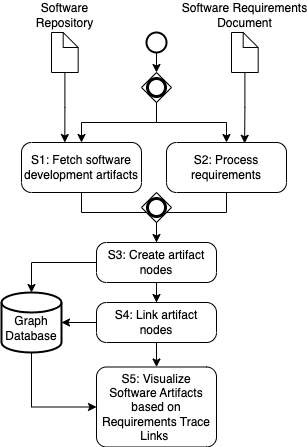
\includegraphics[width=0.65\linewidth]{figs/approach.png}
    \caption{Steps of our approach}
    \label{fig:sys-flow}
  \end{figure}

  The first two steps, \textsf{S1} and \textsf{S2}, concerns processing the two inputs of our approach, a software repository and natural language requirements, respectively. \textsf{S1} fetches issues, pull requests, and commits from a repository whose URL is given. Our prototype expects a Github repository, however our approach is general and can be applied to other repositories where the aforementioned development artifacts are present. %Table~\ref{tab:artifactfeatures} presents the attributes of these artifacts that are used in our approach.
  Our prototype expects a text file containing requirements. It do not enforce a specific for requirements and is able to process the requirements that written in a hierarchical structure, which is a common practice.

          \begin{table}
        \centering
        \caption{Attributes of software development artifacts used in our approach}
        \label{tab:artifactfeatures}
        \begin{tabular}{lllll}
          \toprule
          & Requirement & Issue & PR & Commit \\
          \midrule
          ID &\checkmark &\checkmark&\checkmark&\checkmark\\
          Title &-&\checkmark&\checkmark&-\\
          Description &\checkmark&\checkmark&\checkmark&-\\
          URL&-&\checkmark&\checkmark&\checkmark\\
          Number&\checkmark&\checkmark&\checkmark&\checkmark\\
          State&-&\checkmark&\checkmark&-\\
          Creation Date&-&\checkmark&\checkmark&-\\
          Completion Date&-&\checkmark&\checkmark&\checkmark\\
          Message&-&-&-&\checkmark\\
          Comment Count&-&\checkmark&\checkmark&-\\
          Comment List&-&\checkmark&\checkmark&-\\
          Parent&\checkmark&-&-&-\\
          OID&-&-&-&\checkmark\\
          Text&\checkmark&\checkmark&\checkmark&\checkmark\\
          \bottomrule
        \end{tabular}
      \end{table}


%The tool expects a Requirement Specification Document(RSD) in the form of a text file written in natural language, along with a URL to the GitHub repository of the software project. The software development artifacts, namely Issues, PRs and Commits are fetched from the repository leveraging the GitHub API and the requirement statements are parsed from the given RSD. This operation yields files containing information about Software Development Artifacts (SDA) and requirements, with their associated properties, such as title, description, creation and closure dates, status, and URLs. These artifacts serve as the data source for establishing trace links.

 In \textsf{S3} nodes are created for each of the requirements, issues, pull requests, and commits. 
The features  in Table~\ref{tab:artifactfeatures} are added as the node attributes. 
 Our prototype uses Neo4j\footnote{https://neo4j.com} as a graph database.

      \textsf{S4}  links the requirements to artifacts by creating edges between their associated nodes . 
      Two types of relationships are captured between the artifacts, namely \emph{tracesTo} and \emph{relatedCommit}. 
      The  \emph{tracesTo} relationship represents a trace link between a requirement node and a software development artifact node. 
      The \emph{relatedCommit} is a relation between commit and a pull request nodes. 
      This relation captures provides insight about how the commits are organized by the team. 
      In practice requirements can trace directly to commits or via pull requests (as seen in Figure˜\ref{fig:rawtracegraph}).

      We implement and evaluate three methods to extract trace links, which are represented with the \emph{tracesTo} relation. 
 The first method extracts keywords from the requirements and development artifacts and links the requirements to the artifacts that share keywords. 
 The other methods are based on the \textit{term frequency-inverse document frequency} (TF-IDF) vectors and \textit{word vectors} obtained from a pre-trained model.
For these methods, requirements are linked to the artifacts with similar vectors. 
      The overview of the processing of software artifacts to extract the trace links is shown in Algorithm~\ref{alg:process-software-artifacts}.
            \makeatletter
\algnewcommand\algorithmicswitch{\textbf{switch}}
\algnewcommand\algorithmiccase{\textbf{case}}
\algnewcommand\algorithmicassert{\texttt{assert}}
\algnewcommand\Assert[1]{\State \algorithmicassert(#1)}%
% New "environments"
\algdef{SE}[SWITCH]{Switch}{EndSwitch}[1]{\algorithmicswitch\ #1\ \algorithmicdo}{\algorithmicend\ \algorithmicswitch}%
\algdef{SE}[CASE]{Case}{EndCase}[1]{\algorithmiccase\ #1}{\algorithmicend\ \algorithmiccase}%
\algtext*{EndSwitch}%
\algtext*{EndCase}%
\makeatletter

\setphaserulewidth{0.4pt}

\begin{breakablealgorithm}
\caption{Trace links graph construction}
\label{alg:process-software-artifacts}
\begin{algorithmic}[1]
\State Input: $RSD$ \Comment{Requirement Specification Document}
\State Input: $GRU$ \Comment{Github Repository URL} 
\State Input: $M$ \Comment{Trace Extraction Method} 
\State Input: $\tau_{e}$ \Comment{Threshold for Vector-Based Methods} 
\State Output: $TG$ : \texttt{graph} \Comment{Trace Graph}
\phase{Fetch Software Artifacts}
% \LineComment{Request from Github graphQL API}
\State $\textit{issueList} \hspace{-0.1cm} \leftarrow$  \hspace{-0.2cm} getIssues($GRU$)\label{algl:m}
\State $\textit{prList} \hspace{-0.1cm} \leftarrow$  \hspace{-0.2cm} getPRs($GRU$)\label{algl:m}
\State $\textit{commitList} \hspace{-0.1cm} \leftarrow$  \hspace{-0.2cm} getCommits($GRU$)\label{algl:m}
% \LineComment{Parse directly from given Requirement Specification Document}
\State $\textit{reqList} \hspace{-0.1cm} \leftarrow$  \hspace{-0.2cm} getRequirements($RSD$)\label{algl:m}

\phase{Create Graph with Artifacts}

  \Switch{$s$}
    \Case{$a$}
      \Assert{0}
    \EndCase
    \Case{$b$}
      \Assert{1}
    \EndCase
  \EndSwitch

% \State neo4jConnector($issue_nodes$)\Comment{}

\State $\textit{sdaList} \hspace{-0.1cm} \leftarrow$  \hspace{-0.2cm} $issueList+prList+commitList$\label{algl:m}
% \State $\textit{TG} \hspace{-0.1cm} \leftarrow$  \hspace{-0.2cm} $issueNodes+prNodes+commitNodes+reqNodes$\label{algl:m}
\State $TG \leftarrow$  \texttt{graph} 

\For{\textbf{each} $a$ \textbf{in} sdaList} \label{algl:c}
\State $TG$.addNode(a)
\EndFor \label{algl:c}

\For{\textbf{each} $r$ \textbf{in} reqList} \label{algl:c}
\State $TG$.addNode(r)
\EndFor \label{algl:c}

\phase{Extract Trace Links}

\State preprocess($reqList$, $method$)
\State preprocess($sdaList$, $method$)
\For{\textbf{each} $r$ \textbf{in} reqList}
\For{\textbf{each} $a$ \textbf{in} sdaList}
\If{$method=$ "keyword"}
\State $keywords \leftarrow$ extract(r)
\If{$a.text$ contains any $kw$ in $keywords$}
\State $TG$.addEdge(r,a)
\EndIf
\EndIf
\If{$method=$ "vector-based"}
\State r-v $\leftarrow$ createVector($r.text$)
\State a-v $\leftarrow$ createVector($a.text$)
\If{sim(r-v, a-v)  $\geq$ $\tau_{e}$}
\State $TG$.addEdge(r,a)
\EndIf
\EndIf
\EndFor
\EndFor

\Return $TG$
\end{algorithmic}

\end{breakablealgorithm}

The \textit{getIssues, getPRs, getCommits} functions take a project repository  ($GRU$) and make API calls to the GitHub API\footnote{\url{https://docs.github.com/en/graphql}} to fetch a list of issues, PRs, and commits respectively. 
It fetches the properties shown in Table \ref{tab:artifactfeatures} for these software software artifacts. 
The \textit{$preprocess(list, method)$}  function takes  a list of software artifacts and a method for trace link creation. 
It lemmatizes the text property of each artifact in the list. 
If the method is vector-based then it also removes the stopwords. 
Thereafter, the trace links are determined according to desired method.
In the keyword based method shared keywords between the requirements and software artifacts are sought. In vector based methods the requirements and artifacts are vectorized and their similarities are compared. When similarities exceed a given threshold edges are formed.
For vector-based methods we utilize TF-IDF and word vectors.


% The $sEdge(req, sda, method)$  function determines whether a trace link exists between a given a requirement ($req$) and a software development artifact ($sda$) based on a trace link $method$. If  $method$ is `keyword extraction', the keywords are extracted from $req$ and $sda$ and an edge is created if they share keywords.
% If  $method$ is `vector-based' (tf-idf or word-embedding) vectors are created for  $req$ and $sda$  using their text property. 
% Then, the similarity between the vectors are calculated. 
% An edge is created if similarity value is above a predefined threshold.

 The following details the trace identification methods referred to in the algorithm. %Fig.~\ref{fig:trace-methods} summarizes these three methods to extract trace links.

      % \begin{figure}[htb]
      %   \centering
      %   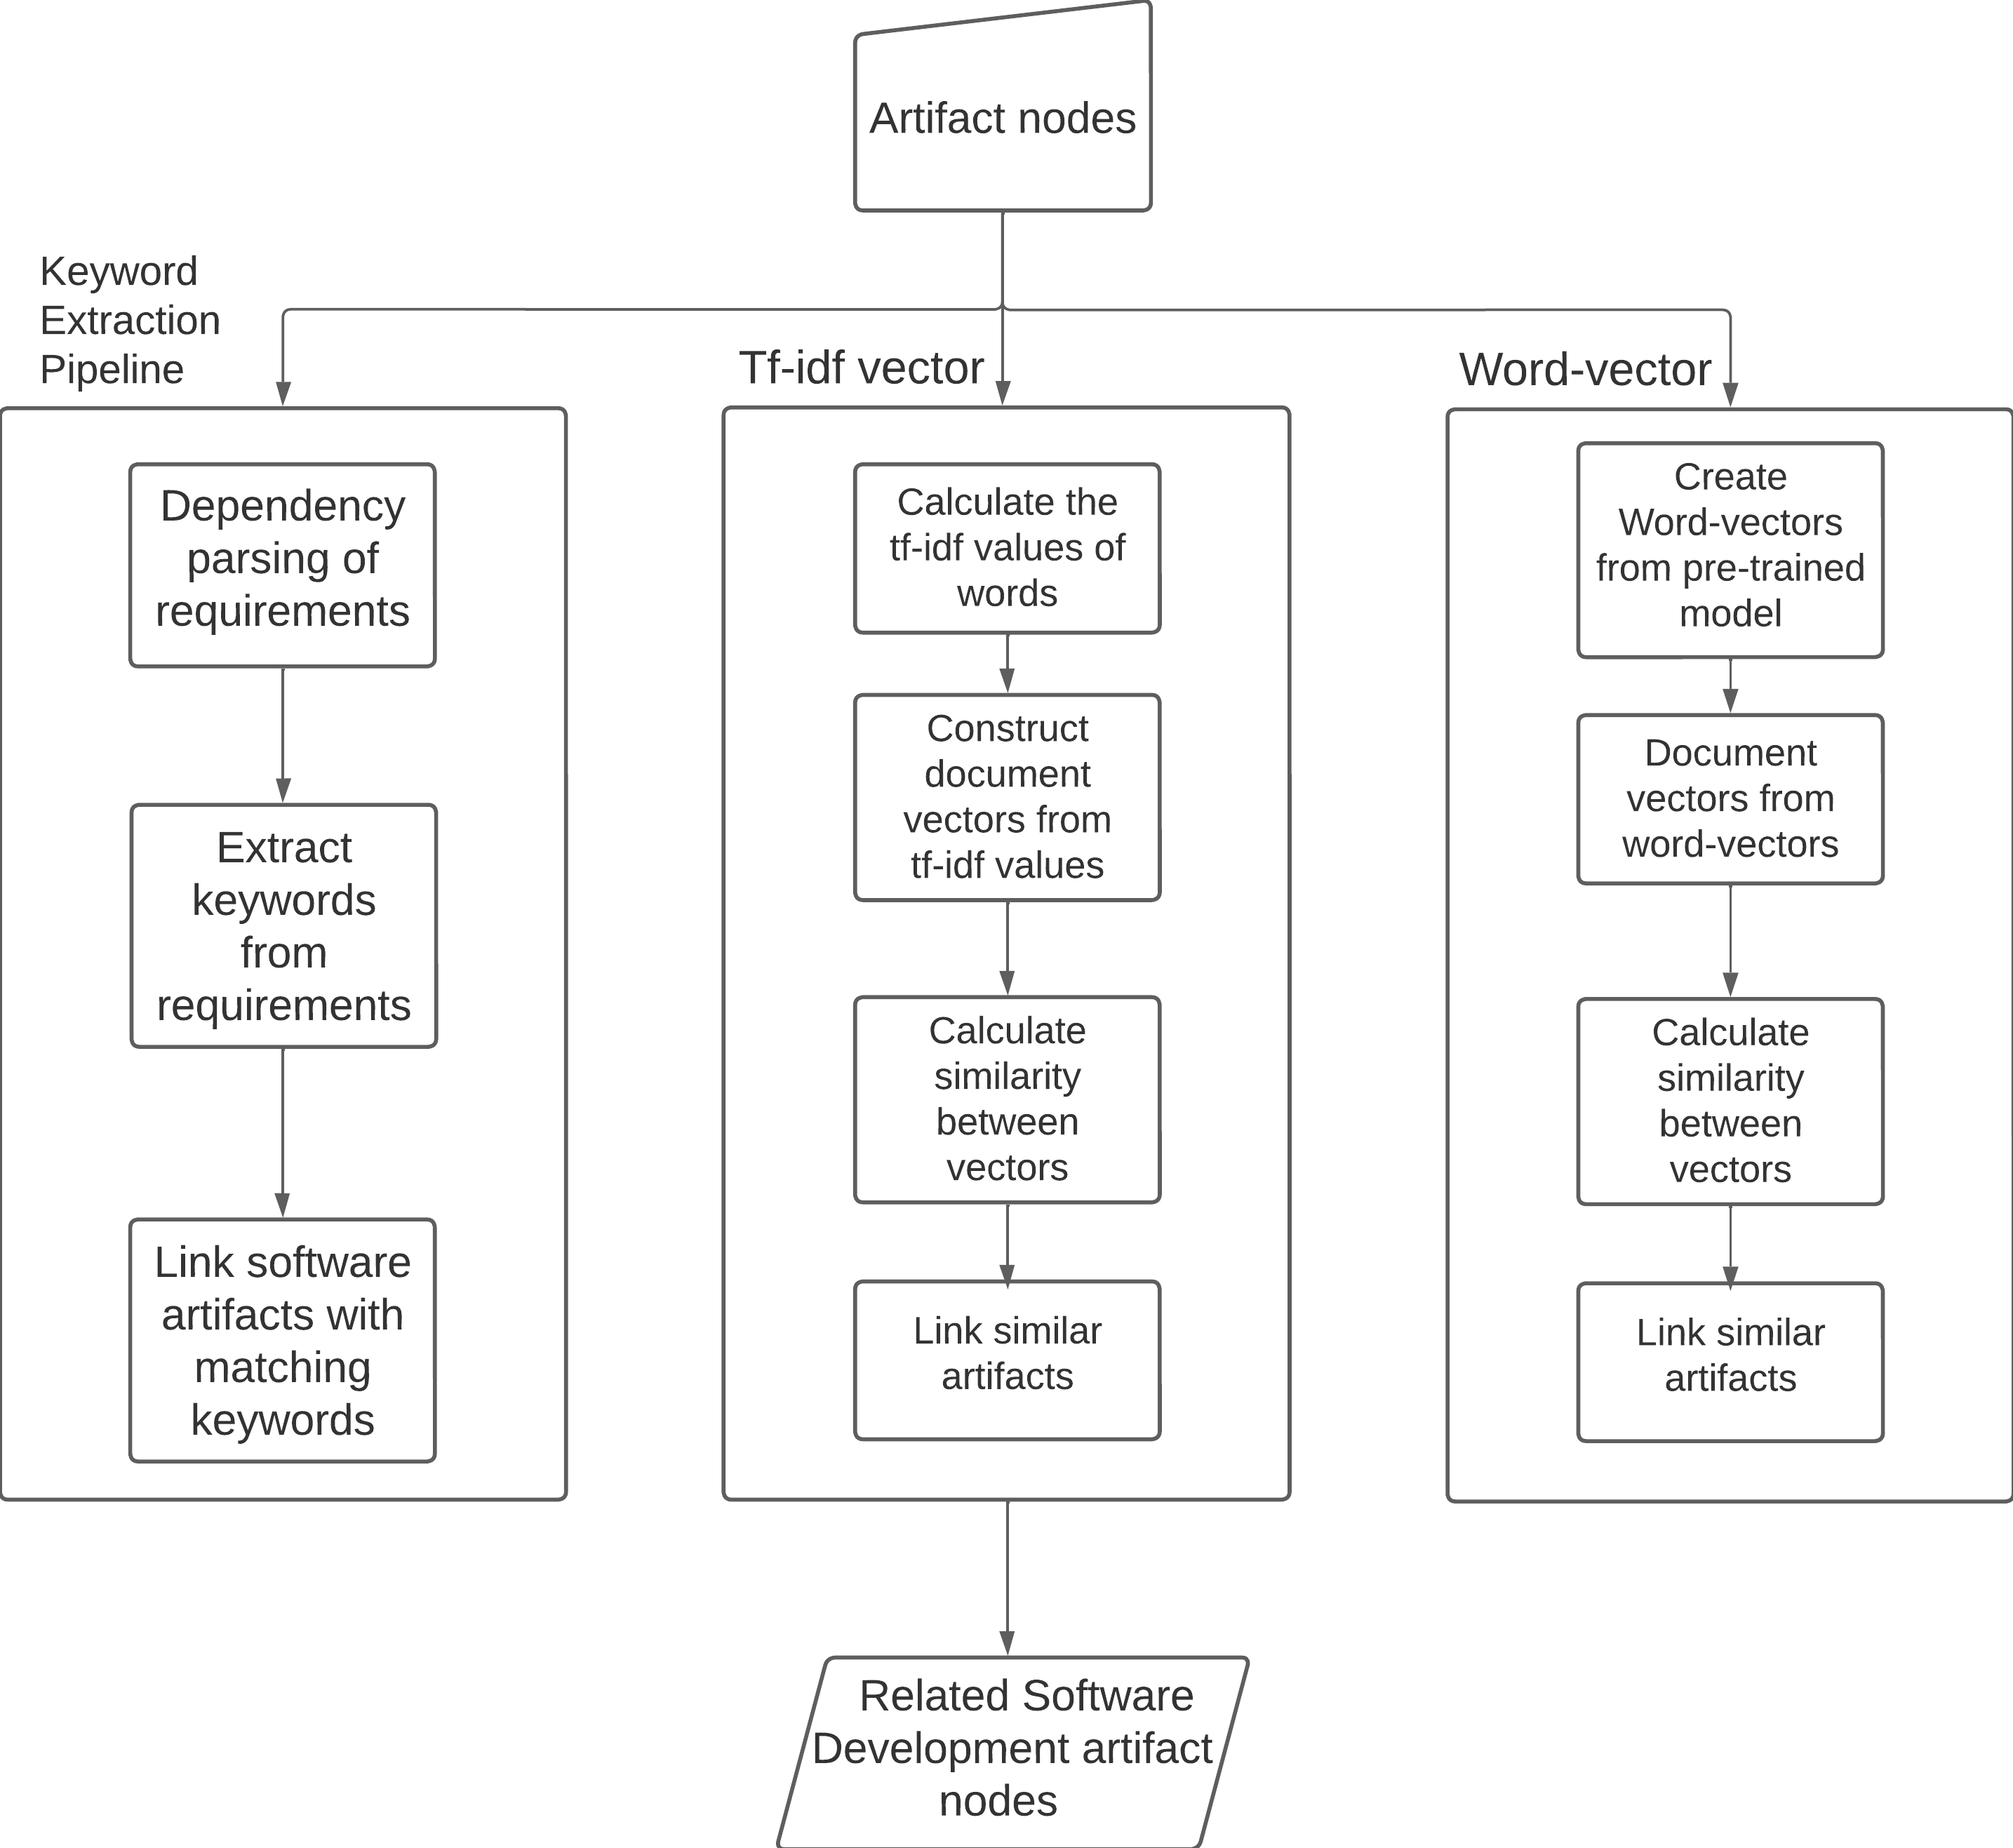
\includegraphics[width=0.9\linewidth]{figs/tracemethods.png}
      %   \caption{Control flow of the trace methods.}
      %   \label{fig:trace-methods}
      % \end{figure}

      \paragraph{Keyword Matching} To identify the most relevant keyword we combine the output of several NLP tasks that are listed below. We identify the keywords from the requirements as our trace link direction is from requirements to the software development artifacts.
      \begin{itemize}
      \item \textit{Tokenization}: We first split the natural language text of requirements.
      \item  \textit{Part-of-Speech Tagging}: We categorize each word to its correct morphosyntactic category by assigning part-of-speech (POS) tags. We focus on nouns, noun phrases, and verbs in our work to identify relevant keywords.

      \item  \textit{Dependency parsing}: We build the dependency trees of sentences to analyze the dependencies between the words of a sentence as shown in Fig.~\ref{fig:deptree}. In this tree structure, we focus on objects and create pairs of verbs and their objects called \emph{verb-objects}, and nouns and their objects called \emph{noun-objects}. We also analyze the indirect objects and conjunctions of the sentences to build these pairs.

      \item  \textit{Stopword removal}: We remove the English stopwords from the pairs we create.

      \item  \textit{Project stopwords removal}: Optionally, we allow the user to select her own stopwords for the project that may not create meaningful links such as the word event for an event management system. In such a project, the word event may create noise for it is likely to be used many requirements and development artifacts.
      \end{itemize}

      % \begin{figure}[htb]
      %   \centering
      %   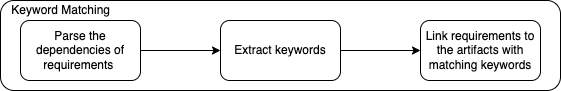
\includegraphics[width=0.99\linewidth]{figs/keywordmatching.png}
      %   \caption{Steps of trace link extraction based on keyword matching}
      %   \label{fig:keymatch}
      % \end{figure}

\begin{figure*}[htbp]
    \centering
    
\includegraphics[width=1\linewidth]{figs/displacy.png}
    \caption{The dependency tree of a requirement.}
    \label{fig:deptree}
  \end{figure*}

  Using these NLP tasks we identify the significant keywords from requirement specifications and prepare a base for identifying trace links. Fig.\ref{fig:keywords} presents the results of the method on an example requirement with the keywords extracted and their labels.

  \begin{figure}[htb]
    \centering
    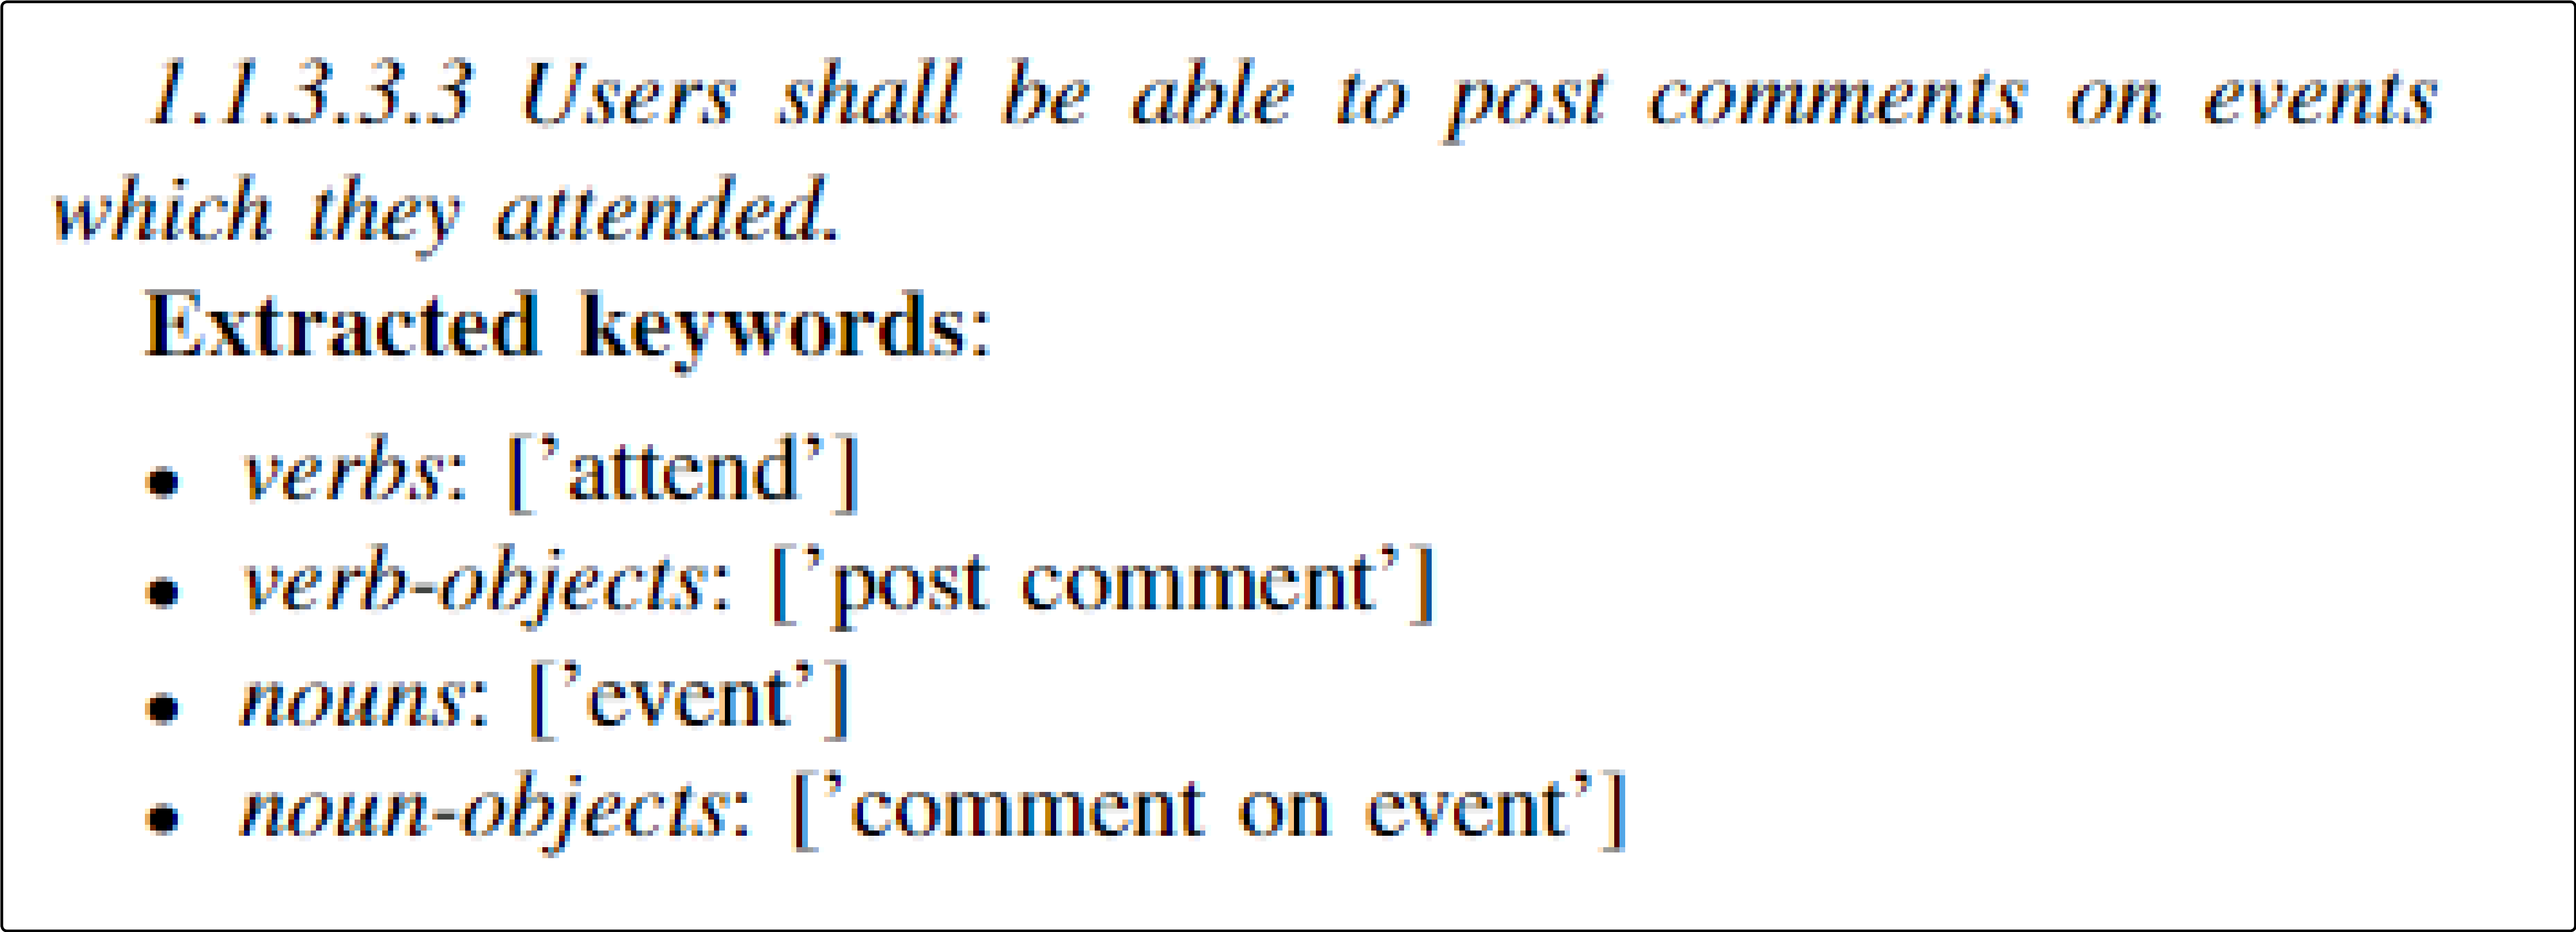
\includegraphics[width=.96\linewidth]{figs/keywords.png}
    \caption{Keyword extraction from a requirement.}
    \label{fig:keywords}
  \end{figure}

  After identifying the relevant keywords of requirements, we match them with the textual attributes of the software development artifacts in the repository. Whe create a trace link when an artifact has at least one matching keyword. We record the link in our graph database by creating an \emph{tracesTo} between the requirement node and the artifact node.

  \paragraph{TF-IDF Vectors} We first build a corpus consisting of all words in the requirements and the software development artifacts. We remove the stop words from this corpus. We calculate the TF-IDF values using Equations \ref{eq:tf}, \ref{eq:idf}, and \ref{eq:tfidf} and construct a TF-IDF vector for each requirement and artifact. We then link the requirements with artifacts that have a similarity score more than a threshold. In Sec.~\ref{sec:eval} we experiment with this threshold. Figure~\ref{fig:tfidfvec} presents the steps for this method.

  \begin{align}
    TF(t,d) &= \frac{\text{frequency of t in d}}{\text{total number of terms in d}} \label{eq:tf} \\
    IDF(t) &= log\frac{N}{1+df} \label{eq:idf}\\
    TF\text{-}IDF(t,d) &= TF(t,d)*IDF(t) \label{eq:tfidf}
  \end{align}

      \begin{figure}[htb]
        \centering
        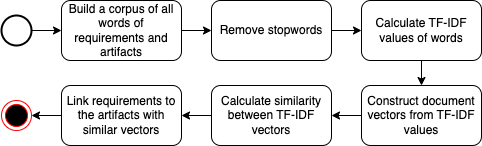
\includegraphics[width=0.99\linewidth]{figs/tfidfvector2.png}
        \caption{Steps for extracting trace links based on TF-IDF vectors}
        \label{fig:tfidfvec}
      \end{figure}

      \paragraph{Word Vectors} To generate word vectors for each artifact we use a pre-trained word embeddings model (word2vec-google-news-300). 
      We gather the word vector for each word within an artifact from the model and to build a vector for each requirement and software development artifact we average the word vectors contained in their textual attributes. 
      To extract trace links for a requirement using TF-IDF and word vectors, we calculate the cosine similarity metric of the requirement's vector with the vectors of other artifacts. 
      The artifacts that have similarities above the decided threshold are recorded as identified traces. 
      Figure~\ref{fig:wordvec} presents this method.

       \begin{figure}[htb]
        \centering
        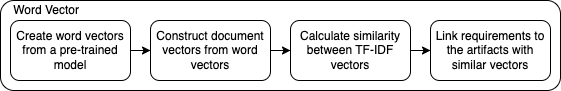
\includegraphics[width=0.99\linewidth]{figs/wordvector.png}
        \caption{Steps of trace link extraction based on word vectors}
        \label{fig:wordvec}
      \end{figure}



\begin{figure}[htb]
    \centering
    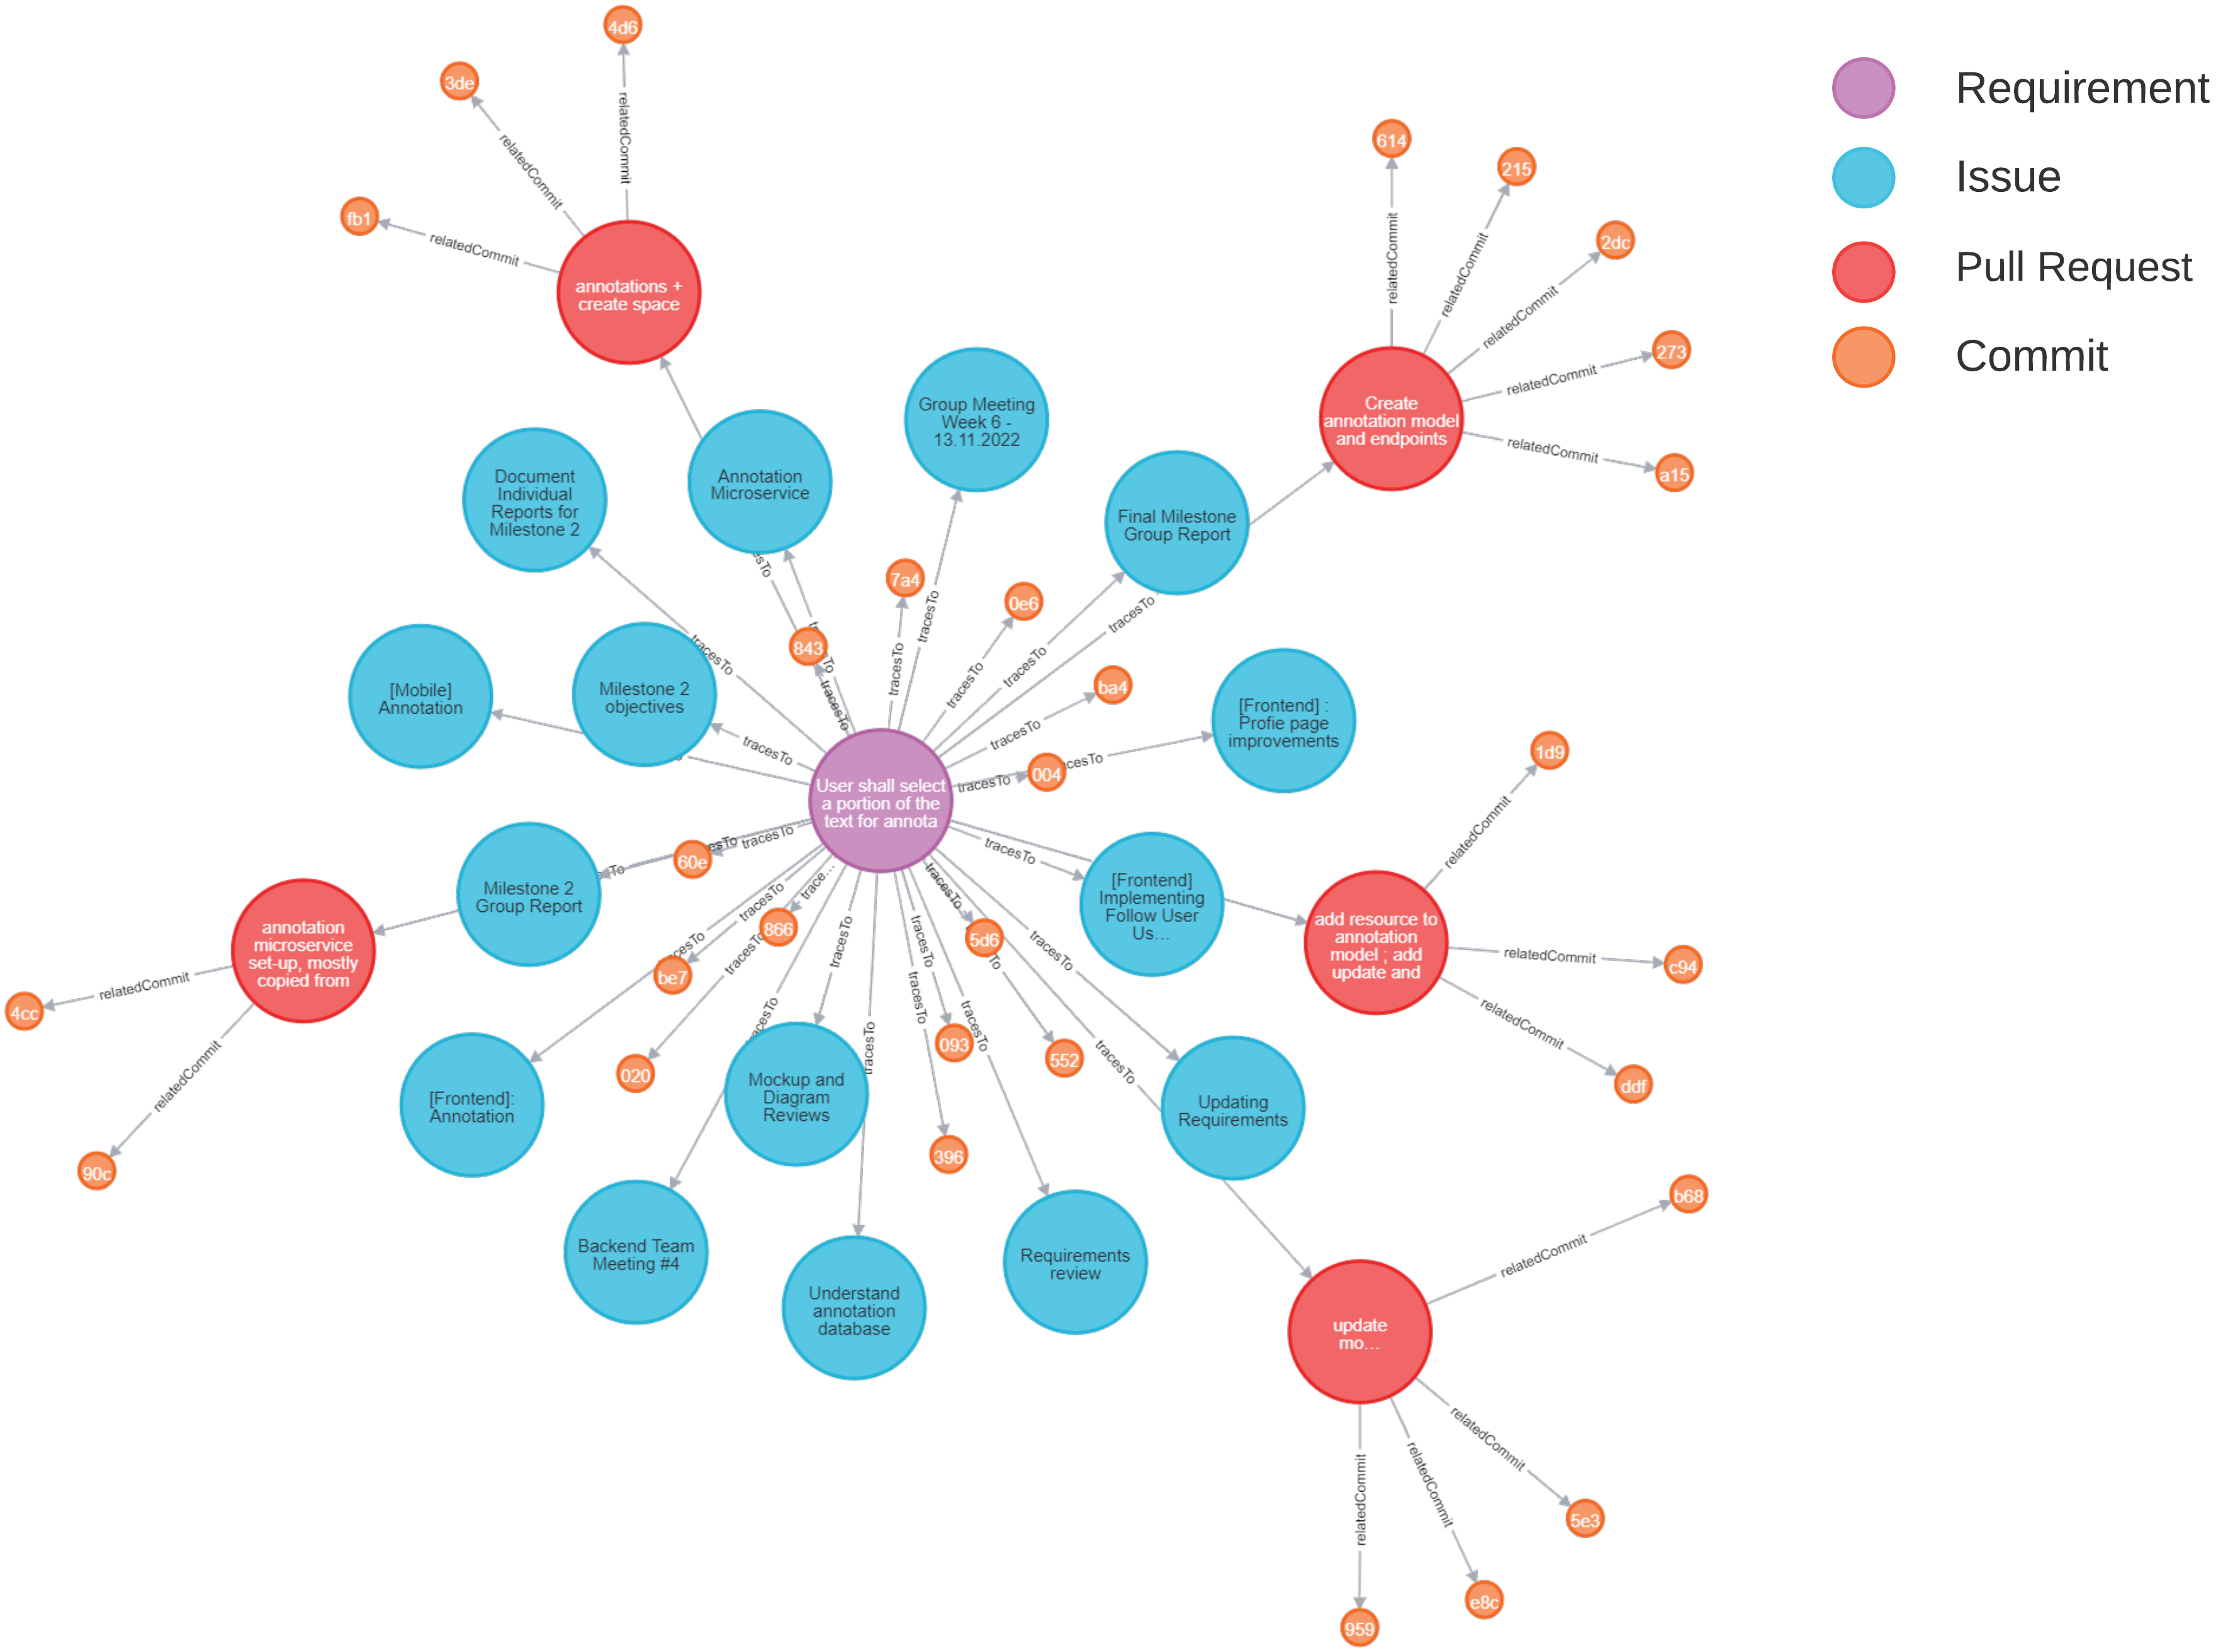
\includegraphics[width=1\linewidth]{figs/rawTraceGraph.png}
    \caption{A segment of a trace graph.}
    \label{fig:rawtracegraph}
  \end{figure}

  We add the \emph{tracesTo} relations to our trace graph based on the extracted trace links. We also add the \emph{relatedCommit} relations between the pull request (PR) nodes and the commit nodes based on the structure of the software repository we analyze. Fig. \ref{fig:rawtracegraph} illustrates a segment of the trace graph obtained from the Neo4j graph database for a specific requirement and displays the associated trace links and related commits.

\begin{figure}[htb]
    \centering
    
\includegraphics[width=.99\linewidth]{figs/traceGraph.png}
    \caption{A segment of a trace graph on a time axis.}
    \label{fig:tracegraph}
\end{figure}

The trace graph itself serves as an effective visualization of the software development artifacts (SDA) that are traced from a requirement. Moreover, it has the potential to display the lifetime of the requirement when the traced SDA are organized chronologically. In Fig. \ref{fig:tracegraph} the related SDA are arranged along a time axis based on their \textit{creationDate} property in order to represent notable information about the stages of implementation. 
For example, it is observed in the figure that the first Pull Request related to the requirement was created in week 8, while the issues concerning the planning of the requirement were created in the early stages of the development. Such visualization is useful during the development phase as well as a retrospective analysis of the software project.




% - The requirement to be examined is the root.
% - The requirement is connected to its related SDAs with \textit{tracesTo} links.
% - Pull request nodes have related commit nodes connected with \textit{relatedCommit} link.

% Who looks at trace?\\
% Trace graph can help a project manager or a developer
% Why?\\
% What can be found?


% A project manager looking at the trace graph can identify:

% \begin{itemize}
%     \item The planning phase of this requirement goes back to week 1
%     \item The implementation of this feature started at week 8
%     \item This requirement took around 13 weeks of work??
%     \item ...
% \end{itemize}

% \pagebreak

% Or in the case of a problem or a bug related to annotation, for example, a developer can view the trace of the requirement about annotation, localizing the search for the problem. Lets say the problem is about updating annotations. Looking at the trace graph, an educated guess can be made, with the information about the problem, to look at a specific pull request. For example, in our case user can view \textit{"Create annotation model"} and \textit{"... add update and delete annotation endpoints..."} nodes. Both nodes can be further observed by using the url property, reaching the github page and examining the code related to them.



Finally, \textsf{S5} provides a visualization where the user can browse the software development artifacts based on the trace links. 
We report several types pf information extracted from the repository to support software development project management. 
Neodash\footnote{\url{https://neo4j.com/labs/neodash/}} is integrated to our Neo4j graph database to provide an interactive dashboard to explore the trace graph.

The dashboard presents information about a software repository and enable the exploration based on trace links.
First, an overview of the software artifacts for a software repository.  
The number of issues and pull requests are visualized in a stacked bar chart per week to view the project progress over time. 
Similarly, the number of  issues closed per week are visualized with stacked bar chart. 
The dashboard also shows the total number of open/closed issues, open/merged PRs, and the average number of trace links per requirement. 
These statistics serve as a snapshot of the current state of the project. 
Fig.~\ref{fig:barcharts} shows the dashboard with for a repository.


%In order to reinforce the visualization of traceability data, our research includes the development of an interactive dashboard, which offers various reports that display statistical insights. Each of these reports was carefully selected to effectively visualize the corresponding data, hence they have user-friendly designs for enhanced comprehension. Moreover, many of these reports are interactive and they allow users to trace the specific requirements, thereby enabling a more customized exploration of the traceability information. The dashboard was implemented using Neodash technology, to provide full integrity with the traceability graph that is stored in the Neo4j database.

% The first report featured in Fig. \ref{fig:barcharts} is a stacked bar chart showing the number of created Issues(in green) and PRs(in brown). It could be observed that the highest number of created artifacts were in week 3 and week 7. The next report is another stacked bar chart that represents the number of artifacts opened and closed per week. Both of these charts are providing information about the status of development in the project lifetime and they help to identify periods of high or low development intensity and let users observe the assessment of the overall project dynamics.

% The dashboard also provides static data regarding the number of open/closed issues, the number of open/merged PRs, and the average number of trace links per requirement. These statistics serve as a snapshot of the current state of the project.

\begin{figure}[hbt]
    \centering
    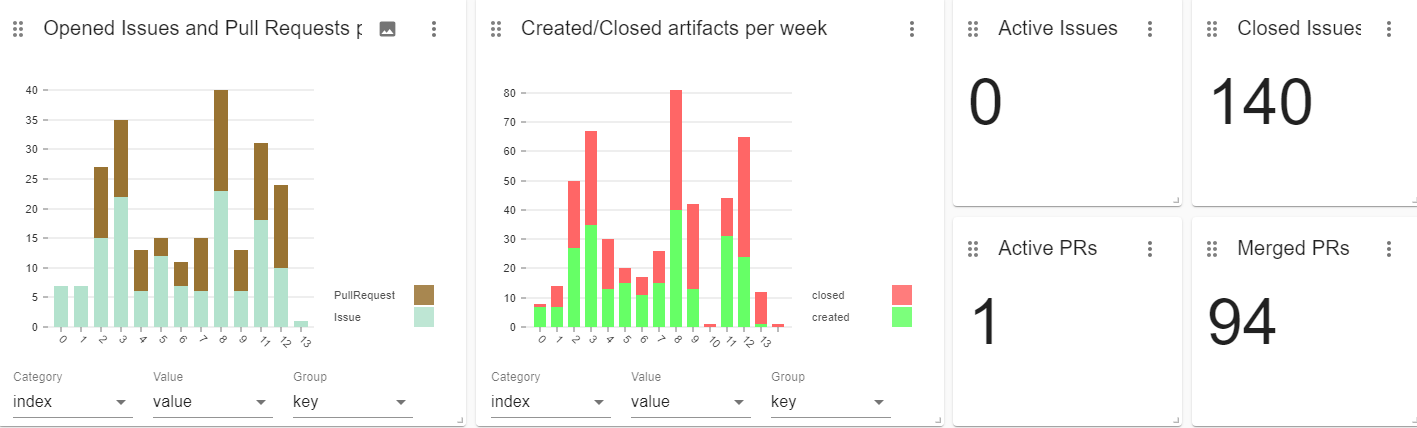
\includegraphics[width=.9\linewidth]{figs/dashboard-barcharts.png}
    \caption{Information about the software artifacts of a project. The first bar chart shows the weekly issues (red) and pull requests (brown) created. The second bar chart shows opened and closed artifacts per week.  On the right, the total number of currently active issues and PRs and completed tasks (issues and PRs). }
    \label{fig:barcharts}
\end{figure}

The dashboard displays the trace links for a requirement over the course of the project on a weekly basis to track the progress of a requirement.
It is presented using a line chart as shown in Figure~\ref{fig:linechart}. 
The project manager can visualize the data of a single requirement or compare the progress of multiple requirements. %By comparing the number of traces for each requirement, the report demonstrates the outliners, that could have relatively less or more traces.
This comparison allows the users to observe the effort associated with each requirement.%
since it displays the number of software development artifacts traced to them.

\begin{figure}[htb]
    \centering
    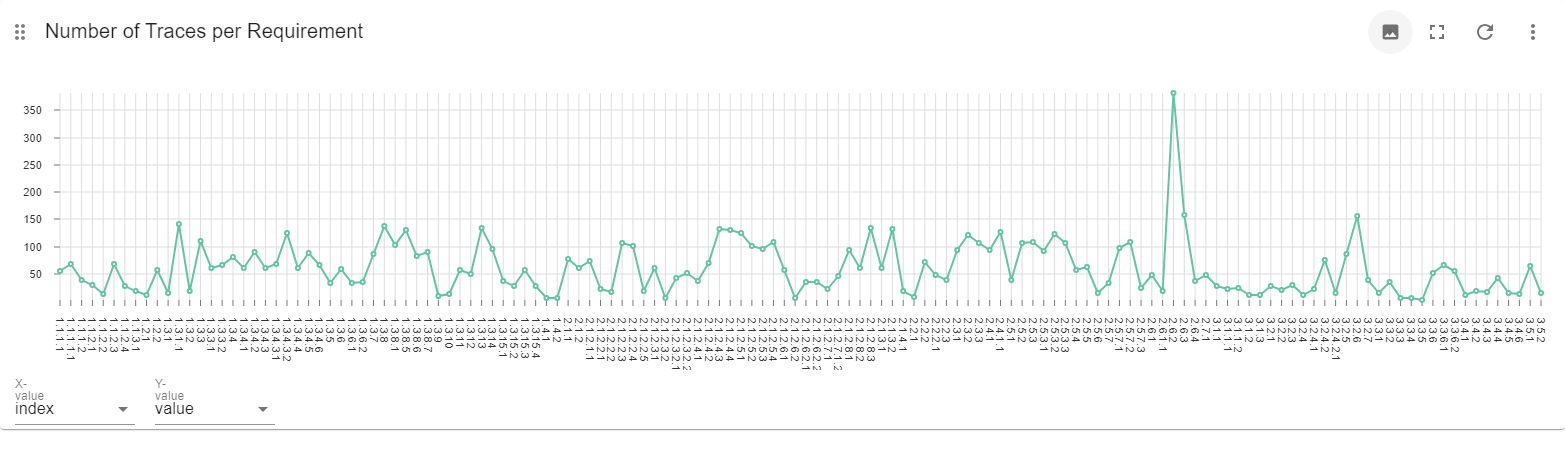
\includegraphics[width=.9\linewidth]{figs/linechart.png}
    \caption{The number of trace links for each requirement. }
    \label{fig:linechart}
\end{figure}

The dashboard shows a comparative  view of two requirements with their weighted relations to software artifacts using  a sankey diagram (Figure~\ref{fig:sankey}). % includes an example of the Sankey chart present in the dashboard that showcases the commonly traced artifacts between the chosen requirements while highlighting the strength of the trace links using the weight property.
Here, thicker lines represent a stronger relations from the requirements to their traced artifacts. 
Thus, one can see how requirements are related via their associated software artifacts.

\begin{figure}[htb]
    \centering
    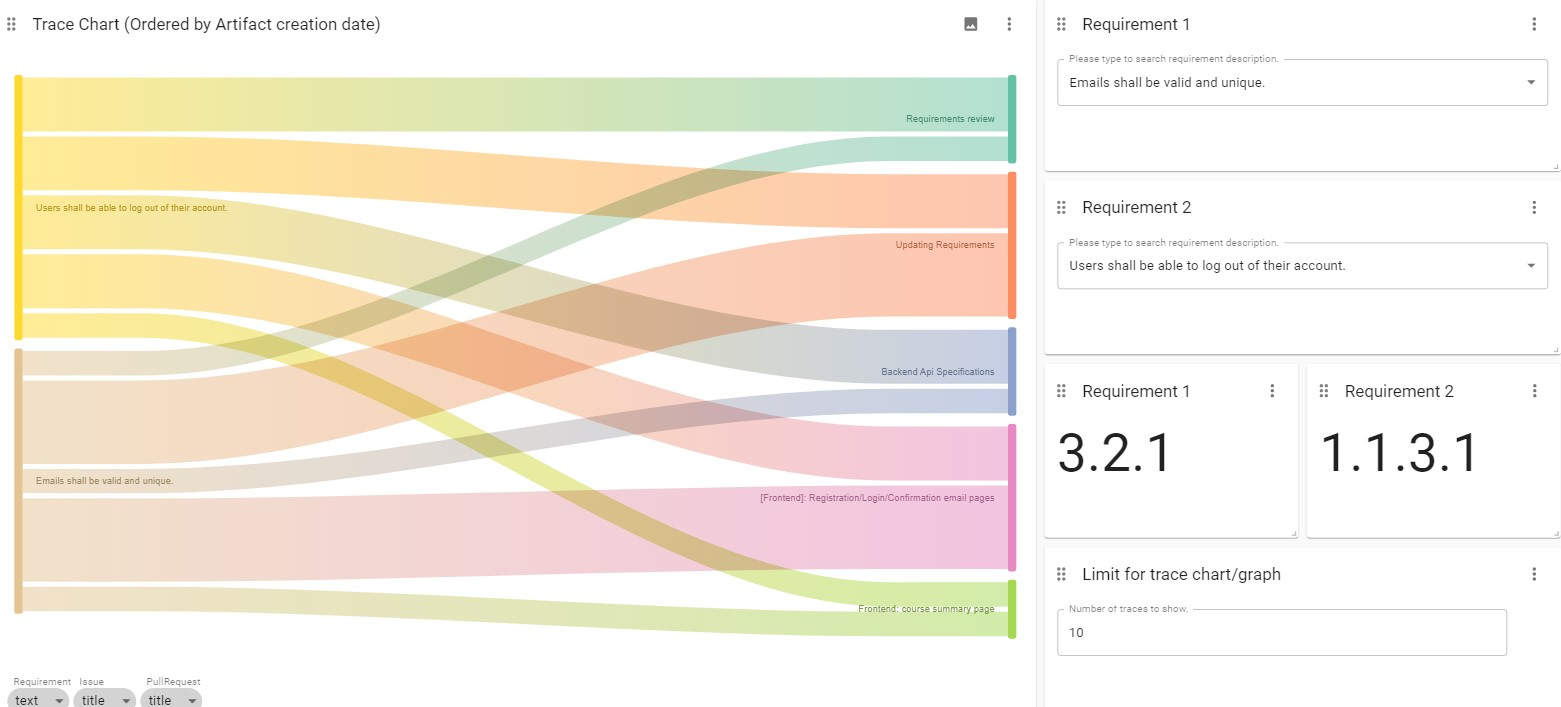
\includegraphics[width=.9\linewidth]{figs/sankey.jpg}
    \caption{The weighted relations between requirements and their associated software artifacts.}
    \label{fig:sankey}
\end{figure}

Users can interact with the dashboard to gain insights on selected requirements as seen in Figure˜\ref{fig:perreq}. 
The identified traces are presented in graphical and tabular formats for  selected requirements.
Their  current status and weekly activities are displayed in the last section of the dashboard.

\begin{figure}[htb]
    \centering
    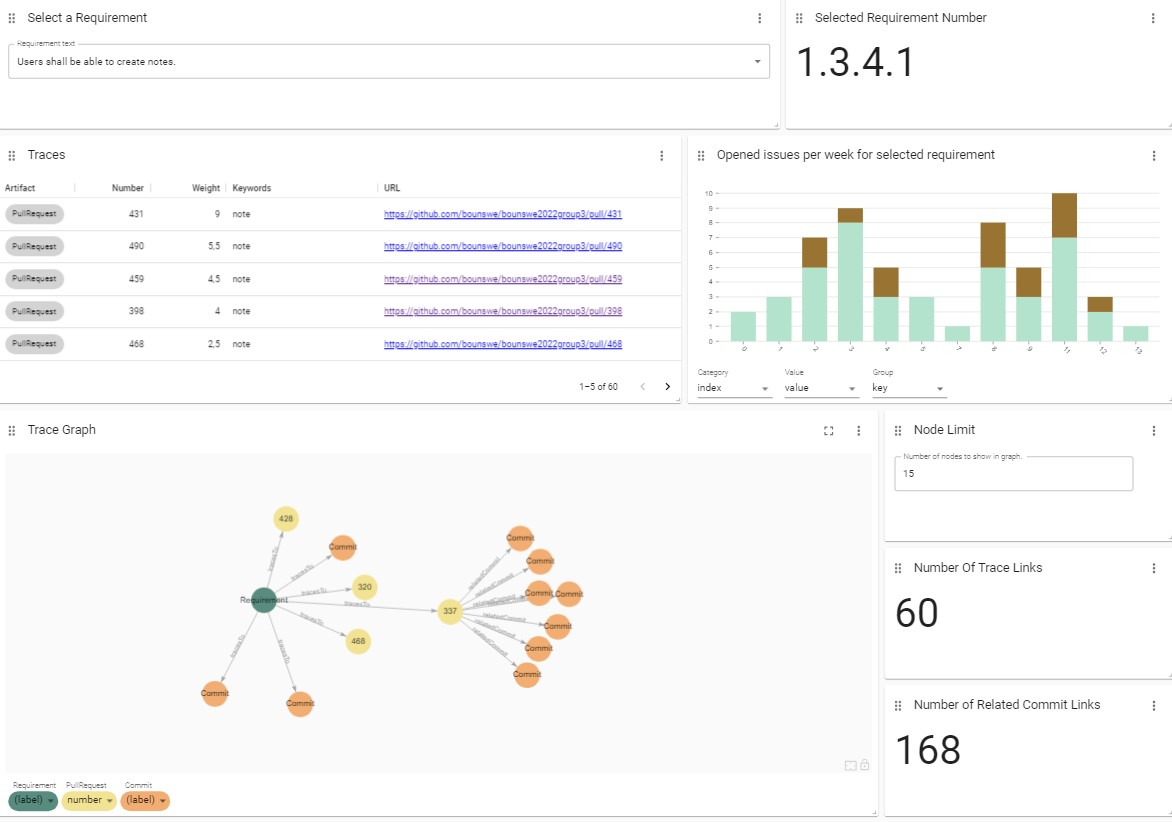
\includegraphics[width=.9\linewidth]{figs/perreq.jpg}
    \caption{Detailed information about a selected requirement.}
    \label{fig:perreq}
\end{figure}

%%% Local Variables:
%%% mode: latex
%%% TeX-master: "../main"
%%% End:

\section{Evaluation}
\label{sec:eval}

% \begin{itemize}
%     \item Ground truth
%     \item Experiment setup
%     \item Results
%     \item Evaluation of results
% \end{itemize}

% This section describes how we evaluated our approach, which focuses on the accuracy of the method utilized in extracting the trace links, namely keyword extraction, TF-IDF vectors and word vectors.

This section presents the results of our preliminary evaluation and detailed evaluation plan for the future.

We evaluate our approach on a public Github repository of a group of computer engineering students for their software engineering course\footnote{Link Anonymized.%https://github.com/bounswe/bounswe2022group2
}. The repository includes the project of an online learning platform. The requirements of the project is also in the repository written in a mixed format where some requirements are written as short phareses to describe a functionality where others as full shall statements. The requirements are structured hierarchically where a parent requirement is further refined into other requirement items.

The first two authors who are familiar with the project but not involved in the project manually extracted the trace links to serve as the ground truth. Below we report the performance of our keyword matching method in Table~\ref{tab:keyperf} and vector-based methods with various similarity thresholds in Table~\ref{tab:vecperf}.

%For this purpose, we selected a set of requirements and thir associated software development artifactsto serve as a ground truth.
%The trace links were manually traced  by our team. \todo{Have we put the selected requirements and traces somewhere? If not let's put it in our repo. }

%The performance of our approach is evaluated using the recall and precision metrics, which inform us about the  percentage of the  traces that were successfully recovered and  the percentage of the traces that are correctly recovered using the following formulas:


%$Recall = \dfrac{True Positives}{True Positives + False Negatives}$


%$Precision = \dfrac{True Positives}{True Positives + False Positives}$


%In the experiment, true positives indicate the trace links that are identified by the method.
%False negatives indicate the trace links that are not identified(missed), and false positives indicate the identified trace %links that are incorrect.
%Table~\ref{tab:keyperf} presents the results of the keyword extraction method and
%Table~\ref{tab:vecperf} shows the results of the vector based methods.


\begin{table}[htb]
\centering
\caption{\label{tab:keyperf}Performance of the Keyword Matching Method}
\begin{tabular}{llll}
  \toprule
  Method & Recall & Precision & F1 Score \\ \midrule
  Keyword extraction & {0.865} & 0.212 & 0.340 \\
  \bottomrule
\end{tabular}
\end{table}

\begin{table}[htb]
\centering
\caption{Performance of the Vector-based Methods}
\label{tab:vecperf}
\begin{tabular}{lllllll}
   \toprule
    \multirow{2}{*}{\shortstack[l]{Similarity \\ Threshold}}
  & \multicolumn{3}{c}{Word-vector} &  \multicolumn{3}{c}{TF-IDF vector} \\
   \cmidrule{2-7}
                                                          & {Rec.} & {Prec.} & F1 &  {Rec.} & {Prec.} & F1\\
   \midrule
  0.05 & 1 & 0.043 & 0.082 & 0.839 & 0.121 & 0.211 \\
  0.15 & 1 & 0.043 & 0.082 & 0.573 & 0.256 & 0.354 \\
  0.25 & 1 & 0.043 & 0.082 & 0.244 & 0.43 & 0.311 \\
  0.35 & 1 & 0.043 & 0.082 & 0.095 & 0.392 & 0.153 \\
  0.45 & 0.965 & 0.071 & 0.132 & 0.025 & 0.125 & 0.042 \\
  0.55 & 0.865 & 0.1 & 0.179 & 0.013 & 0.121 & 0.023 \\
  0.65 & 0.294 & 0.3 & 0.297 & 0 & 0 & -- \\
   \bottomrule
 \end{tabular}
\end{table}

Based on the F1-scores, TF-IDF vector based method has the best F1 score followed by the keyword matching method on this repository followed by keyword matching method. The performance of the vector-based methods  significantly varies according to the threshold value. Setting a low thresholds links requirements with many artifacts yet few of these links are actually valid.


%The recall values  approach 1 with low  threshold values which also yield significantly low precision values.
% This indicates that the desired traces are recovered, but also that,  almost all of the SDAs have been identified as candidate traces.
% On the other hand, high threshold values result in the  opposite,yielding low recall and higher precision values.
% Notably, the word vector method achieved the highest precision value among the results when the threshold was set to 0.25.

% In conclusion, these results indicate that each method its strengths, and selecting the most suitable among them is dependent  on the specific project structure and requirements. \todo{I don't find this convinging argument. What kinds of structured would we prefer which methods for? Like what structure? It may depend more on how the project team documents its work as the traces are captured from the articulation of the team members and their code conventions (variable names, commenting etc.)}

We do not reach any conclusions based on our preliminary evaluation. This evaluation demonstrates that our approach is applicable for tracing requirements in a software repository but we refrain ourselves to be conclusive on the performance of the methods. In the near future we plan two additional evaluation studies.

The first study concerns the evaluating our approach again in educational setting where we analyze the repositories of student groups, report on perceived usefulness and usability of our dashboard study any correlations with the statistics reported by our dashboard and the performance of the groups in the course.

The second study is a case study with an industry partner where we ask for the ground truth from the experts from the industry and report the performance of different methods to extract trace links as well as perceiived usefulness and usability of our dashboard in comparison to trace matrix, which is widely used in the industry for tracing requirements.

%%% Local Variables:
%%% mode: latex
%%% TeX-master: "../main"
%%% End:

\section{Discussion}
\label{sec:discuss}

\emph{Observations.} Our experiments on the evaluation of the tool have led us to observe that the quality and consistency of the requirement statements and the software development artifacts (SDA) significantly impact the effectiveness of our approach in identifying trace links. Well-written requirement specifications that are self-explanatory and granulated lead to better performance of its traces along with software development artifacts that have textual data (e.g. title, description, comments) that is semantically related to the feature they implement.

\emph{Limitations.} The current implementation of our approach traces requirements to issues, pull requests, and commits. A more thorough trace should include other artifacts such as the architecture models, code, and test cases. Our implementation handles English only, other languages are not supported. The keyword matching method focuses on the syntax rather than the semantics of the word, yet consistent use of terms and agreeing on a glossary should mitigate this limitation.

\emph{Implications in practice.} Our approach aims to visualize software repositories based on trace links. Improving the performance of trace link extraction would provide more accurate data for the dashboard visualization. We hypothesize that software engineering educators and students can benefit from this visualization to track the progress of the software projects both during and after the development phase. Visualization of traces of a requirement presents the maturity of the implementation of a requirement and the contribution patterns of students. Similarly, companies can track the progress of their projects and can gain retrospective insights on projects for good and bad practices based on the visualizations provided in our dashboard.

\emph{Threats to validity.} Our evaluation presented in this paper is preliminary. To mitigate the threats to internal validity, we selected a repository the authors were not involved and two authors collaborated on building the ground truth to reduce personal bias. We cannot reach any conclusions about the external validity of the results. We need to conduct more studies to generalize the results. We share our replication package and invite the community to replicate our work for reliability.
\section{Conclusions}
\label{sec:conc}

In this paper, we presented a tool that automates the traceability link recovery by identifying trace links between requirements written in natural language and software development artifacts(Issues, PRs, Commits) obtained from GitHub repositories. Through the implementation of three optional methods, namely keyword extraction, TF-IDF vector and word vector, we have demonstrated the capability of identifying traceability links of our tool. We have stored the traceability data we obtained in a graph database to visualize the trace links, and supported the data with an interactive dashboard, which provides users with comprehensive statistical insights.

In conclusion, our tool provides an automated solution for requirement traceability(RT) and enhances the management of software projects. By optimizing the time and effort required for RT and offering educational opportunities for project management, our tool contributes to the overall success of software development projects. With future development and evaluation, our study carries the potential to positively impact traceability practices.










\bibliographystyle{IEEEtran}
\bibliography{paper}
\end{document}


%%% Local Variables:
%%% mode: latex
%%% TeX-master: t
%%% End:
